\documentclass[letterpaper, 12pt]{article}
\usepackage[letterpaper, top=2.5cm, bottom=2.5cm, left=3cm, right=3cm]{geometry} %margenes
\usepackage[utf8]{inputenc} %manejo de caracteres especiales
\usepackage[spanish]{babel} %manejo de encabezados de inglés a español
\usepackage{fancyhdr} %formato de los encabezados de página
\usepackage{ragged2e} %alineado real justficado
\usepackage{graphicx} %manejo de imagenes
\usepackage{amsmath} %manejo de notación matemática
\usepackage{mathtools} %manejo de notación matemática
\usepackage{blindtext} %texto de relleno
\usepackage{cancel} %permite la simbolización de cancelación de terminos
\usepackage{enumitem}[shortlabels] %listas con letras
\usepackage{amssymb} %manejo de simbolog►1a matematica
\usepackage{float}

\pagestyle{fancy}
\fancyhf{}
\rfoot{\thepage}

\begin{document}
\setcounter{page}{1}
\thispagestyle{fancy}
\lhead{\textbf{Tarea 2, U4}}
\rhead{\textbf{2 de diciembre del 2020}}
\section*{Funciones reales de varias variables}
\subsection*{Dibujar las siguientes curvas de nivel}
\[\begin{matrix}
    x+2y=-2\\
    x+2y=-1\\
    x+2y=0\\
    x+2y=1
\end{matrix}\]
\subsection*{Gráfica}
Cada una nos da planos con cierta separación cada uno.
\begin{figure}[H]
    \centering
    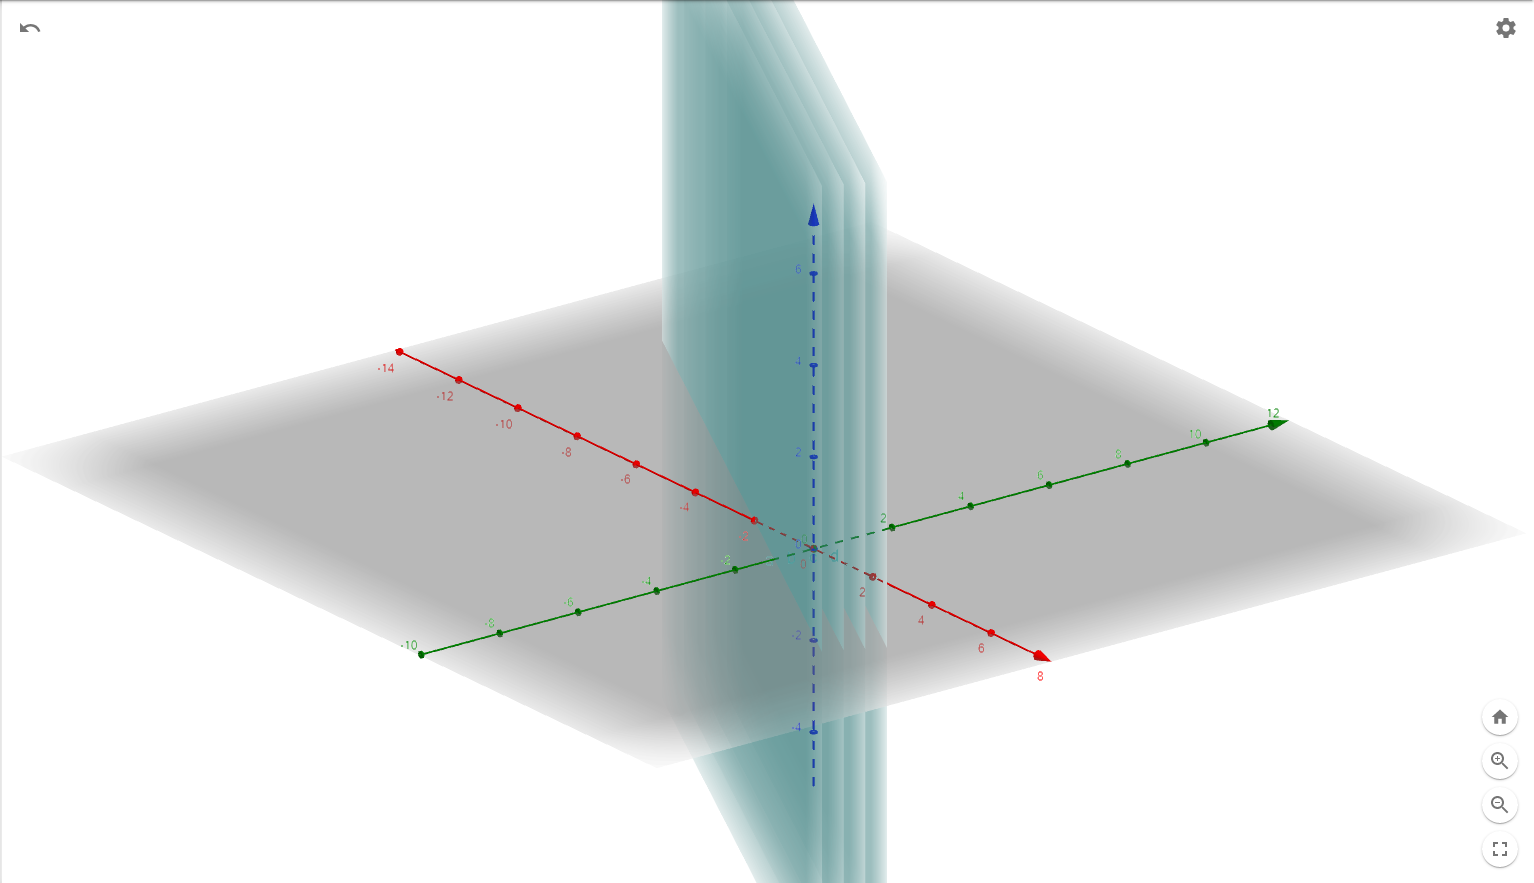
\includegraphics[width=12cm]{grafica.PNG}
\end{figure}
\end{document}